%========================================================================================
% TU Dortmund, Informatik Lehrstuhl VII
%========================================================================================

\chapter{Probleme und L{\"o}sungen}
\label{Probleme_und_Loesungen}
%
Im folgendem werden einige Probleme, die bei der Implementierung des Projektes aufgekommen sind, beschrieben und des weiteren werden verschiedene L{\"o}sungsans{\"a}tze dazu vorgestellt.

\section{Bewegung der Schlange}
\label{Bewegung der Schlange}
%
Bei der Implementierung der Schlange wurde am Anfang erst ein Quadrat erstellt, danach musste die Bewegung hinzugef{\"u}gt werden. Da am Anfang noch keine Bildschirmrate gab, konnte die Schlange in jede Richtung in Echtzeit laufen, je nach Eingabe der Richtung. Um die Schlange in direkter Diagonalen Richtungen zu vermeiden, wurde die Bewegung in Horizontaler- und Vertikaler-Achse beschr{\"a}nkt. Das Problem war, dass die Schlange in die entgegengesetzte Richtung laufen kann, d.h. die Schlange konnte durch sich selbst durchlaufen.

Der erste L{\"o}sungsansatz war mit Hilfe von einer Variable die aktuelle Richtung zu speichern um je nachdem in die andere Achse zu laufen. Damit wird verhindert direkt in die entgegengesetzte Richtung zu laufen. Jedoch wurde das Problem noch nicht behoben, da durch das gleichzeitige Benutzen von mehreren Richtungseingaben die Variable eine falsche Richtung erh{\"a}lt und somit die entgegengesetzte Richtung erlaubt. Dies kann so schnell passieren, sodass die Schlange die zweite Richtung nicht wahrnimmt und sofort in die entgegengesetzte Richtung l{\"a}uft.

Deshalb gab es einen endg{\"u}ltigen L{\"o}sungsansatz, welcher mit zwei Variablen und mit der Methode, die jeden Schritt der Schlange verarbeitet, arbeitet. Die Variablen sind dabei einmal $p1Direction$ (f{\"u}r Player1 und Player2 $p2Direction$) f{\"u}r die aktuelle Richtung und $p1NextDirection$ (f{\"u}r Player1 und Player2 $p2NextDirection$) f{\"u}r die n{\"a}chste Richtung. Die Idee mit dem Verhindern der Achse bleibt. Jedoch wird die aktuelle Richtung erst auf die neue Richtung gesetzt, sobald die Schlange sich um ein Feld bewegt. 
%
\section{Elemente Erzeugen}
\label{Elemente Erzeugen}
Relativ fr{\"u}h in der Entwicklung des Spiels machten sich Performanceprobleme beim Erstellen neuer Elemente, vor allem des $foodElement$, bemerkbar. Bei zunehmend langer Schlange erh{\"o}hte sich die Rechenzeit f{\"u}r das Finden einer freien Stelle auf dem Spielfeld so stark, dass zum Beispiel nach dem finden des $foodElements$, eine bemerkbare Pause entstand in der das Spiel nicht weiterlief und somit stockte. Diese Pause war allerdings nicht gleichbleibend lang, sondern erschien zuf{\"a}llig und mit unterschiedlicher Dauer, jedoch mit ansteigender L{\"a}nge der Schlange {\"o}fter und mit erhöhter Dauer.\\
Dies war zur{\"u}ckzuf{\"u}hren auf unseren Algorithmus zur Bestimmung einer freien Stelle sowie die Speicherung der Schlange in einer Liste. Der Algorithmus suchte pseudo-randomisiert eine Stelle des Spielfeldes aus und {\"u}berpr{\"u}fte daraufhin, ob ein Element der Schlange bereits auf diesem Feld ist. Falls dies nicht der Fall war, war das Feld geeignet, ansonsten wurde einfach ein anderes Feld ausgesucht und dies solange wiederholt bis ein freies Feld gefunden wurde. Durch eine l{\"a}ngere Schlange stieg somit die Wahrscheinlichkeit, dass ein neues Feld ausgesucht und der {\"u}berpr{\"u}fungsprozess deshalb mehrere Male durchgef{\"u}hrt werden musste. Das gr{\"o}ßere Problem hierbei war aber der {\"U}berpr{\"u}fungsprozess selber, sowie die Speicherung der Schlange in einer verketteten Liste. Um zu {\"u}berpr{\"u}fen, ob das ausgesuchte Feld nicht schon durch die Schlange belegt war, musste die gesamte Schlange Element f{\"u}r Element {\"u}berpr{\"u}ft werden. In Kombination mit der Wahrscheinlichkeit auf mehrere {\"U}berpr{\"u}fungen entstand dadurch bei l{\"a}ngeren Schlangen ein so großer Rechenaufwand, dass die  Verz{\"o}gerung durch den Spieler bemerkbar und somit der Spielfluss ins stocken geraten ist.\\
Zur L{\"o}sung des Problems wurde eine neue Variable eingef{\"u}hrt, welche auch in der weiteren Entwicklung noch sehr hilfreich wurde: ein zweidimensionales Array mit Integer-Werten, das $fieldArray$. Das $fieldArray$ dient als kompakte Darstellung des aktuellen Zustands des gesamten Spielfelds. Dabei repr{\"a}sentierte jeder der 39 x 29 Integer-Werte eine Stelle auf dem Spielfeld und deren aktuellen Zustand. Ist der Wert 0 ist das Feld frei, ist der Wert 1 ist die Stelle von der Schlange von Spieler 1 belegt usw. . Alle Werte und zugeh{\"o}rigen Zust{\"a}nde sind in Tabelle \ref{tbl:Fieldarray-Werte}zu sehen.
\\
Durch das $fieldArray$ ist nun der Prozess des {\"u}berpr{\"u}fens einer Stelle nicht mehr abh{\"a}ngig von der L{\"a}nge der Schlange, sondern kann immer in konstanter Zeit durch einmaliges checken des zugeh{\"o}rigen Wertes im $fieldArray$ erledigt werden. Das Problem der mehrmaligen {\"u}berpr{\"u}fungen durch Ausw{\"a}hlen eines bereits belegten Feldes ist damit auch trivialisert, da das {\"u}berpr{\"u}fen nun schnell genug geht. Durch das $fieldArray$ wurde auch die weitere Implementierung des Spiels vereinfacht, da durch neue Wertezuweisungen im Array relativ einfach neue Objekte wie W{\"a}nde und PowerUps in die Spiellogik eingef{\"u}hrt werden konnten, und das {\"u}berpr{\"u}fen der Stellen an denen diese Objekte sich befinden durch das $fieldArray$ direkt abgedeckt ist.

\begin{minipage}[X]{1.1\textwidth}
 \centering
 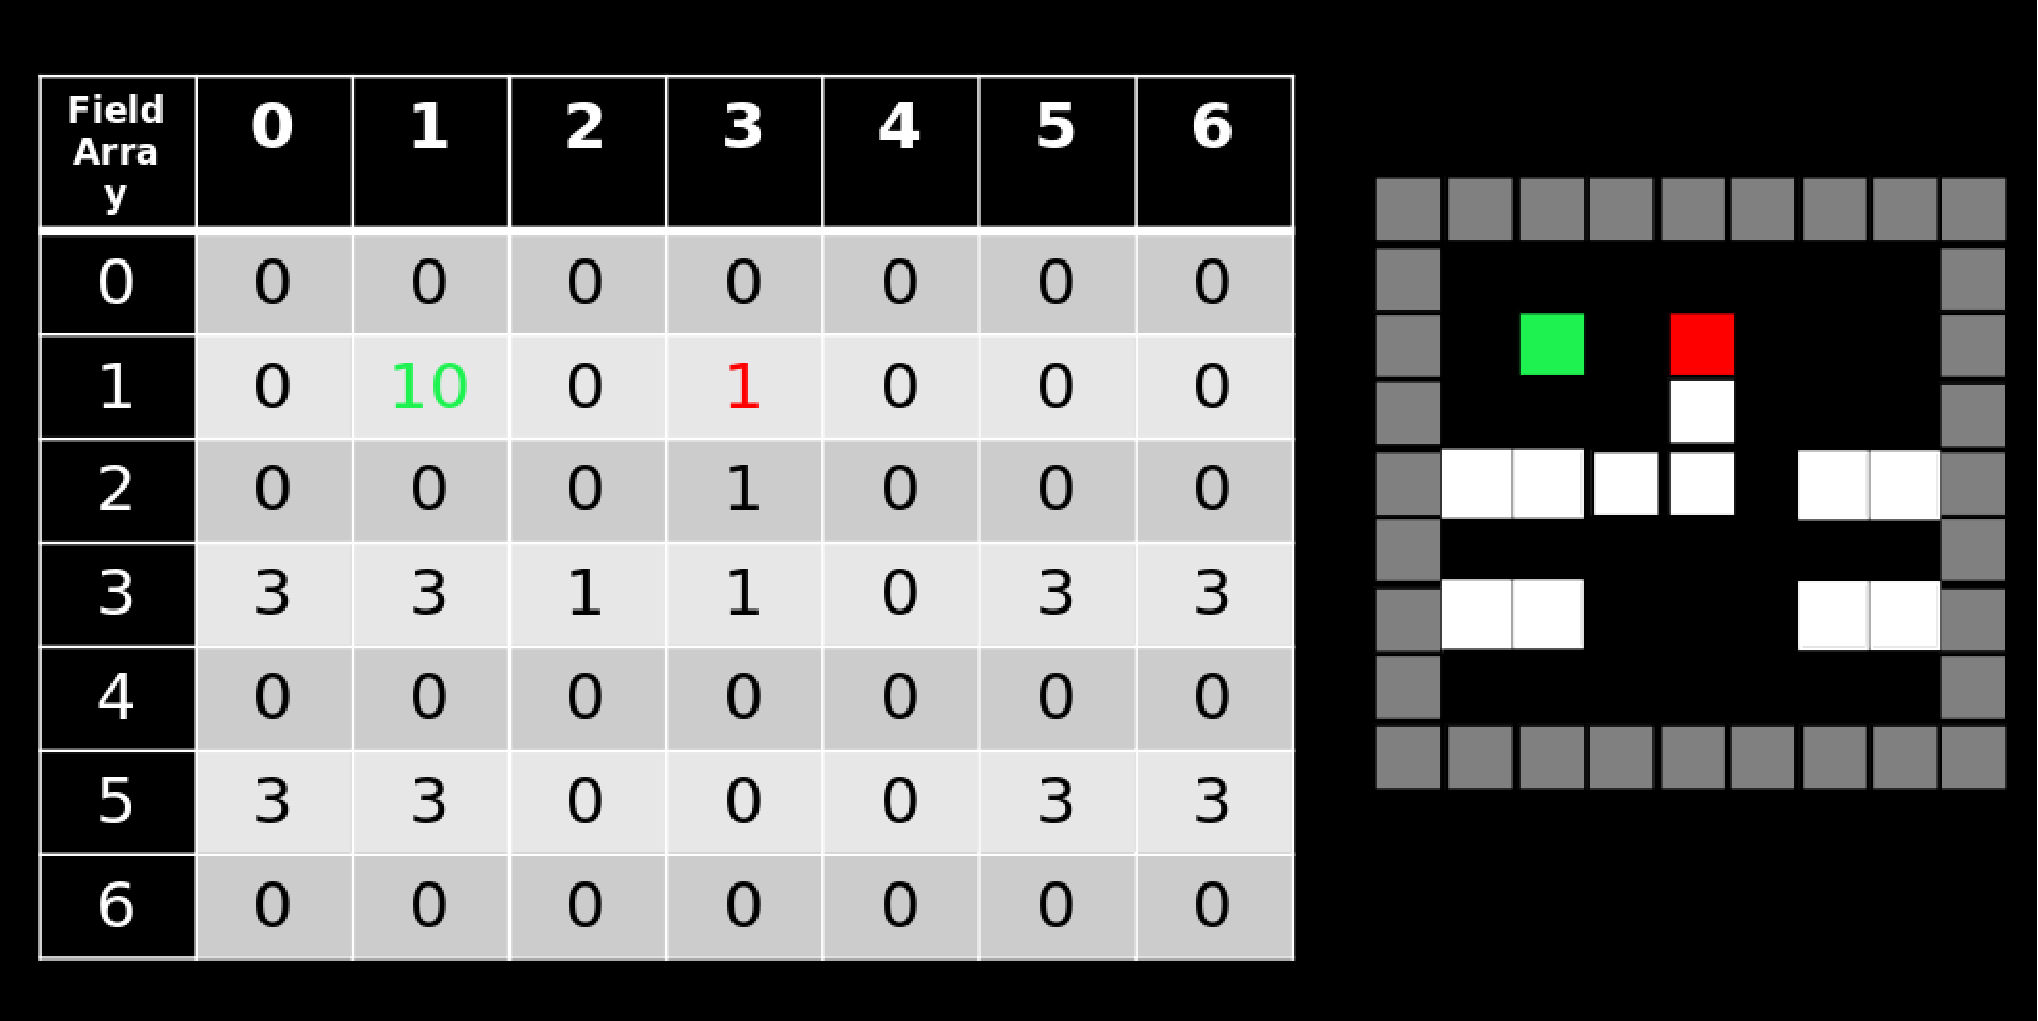
\includegraphics[scale=0.3]{bilder/FieldArraySpielfeld}
 \captionof{figure}{Darstellung des eines Spielfeldes mit dazugehörigem $fieldArray$}
 \label{fig:FieldArraySpielfeld}
\end{minipage}


\begin{table}
     \centering
     \begin{tabular}{ll}
       \textbf{Wert}  & \textbf{Objekt} \\
       0          & Leer                 \\
       1         & Spieler 1             \\
       2         & Spieler 2             \\
       3         & Wand                 \\
       10        & Food-Element             \\
       11        & Superfood-Element             \\
       12        & Freeze-Element             \\
       13        & Reduce-Element             \\
       14        & Inverse-Element             \\
       20        & Teleport             \\
     \end{tabular}

     \caption{Fieldarray-Werte}
     \label{tbl:Fieldarray-Werte}
     % Verweis im Text mittels \ref{tbl:beispieltabelle}

   \end{table}




%
\section{Spielleistung}
\label{Spielleistung}
%
Beim Ausf{\"u}hren des Spiels kam es sehr oft zu Problemen mit der Spielleistung. Insbesondere wenn das Spiel mit anderen Programmen, wie BigBlueButton, gleichzeitig lief. Dies f{\"u}hrte in den meisten F{\"a}llen zur Verlangsamung des Spielfluss. Desweiteren flackerte das Spiel sehr stark, sodass {\"a}ltere Frames anstatt des neuen Frames gezeichnet wurden. Weitere Probleme waren h{\"a}ufig auftretende Speicherzugriffsfehler vor allem, wenn das Spiel {\"u}ber eine virtuelle Maschine lief. Jener Fehler f{\"u}hrte zur Terminierung des Spiels.  
%
